\documentclass[12pt]{article}
\usepackage{graphicx} % Required for inserting images
\usepackage[a4paper, top=0.5cm, left=2cm, right=2cm,bottom=2cm]{geometry}
\usepackage{amsfonts}
\usepackage{amsmath}
\usepackage{mathtools}
\usepackage{amssymb}
\usepackage{multicol}
\usepackage{fullpage}
\usepackage{graphicx}
\usepackage{float}
\usepackage{pgfplots}
\usepackage{tikz}

\geometry{top=1.2cm}
\title{\small Facultad de Matemática, Astronomía, Física y Computación}
\author{Simulacro Segundo Parcial\\ GURI - La Bisagra, conduccion del CEIMAF}
\date{}
\begin{document}
\maketitle
\begin{enumerate}
    \item 
    \begin{enumerate}
        \item Primero trabajemos con la recta $L$ escribiéndola de la forma $mx+b$:
        \begin{equation*}
            L:y=\frac{2}{3}(x-2)+2=\frac{2}{3}x-\frac{4}{3}+2=\frac{2}{3}x+\frac{2}{3}
        \end{equation*}
        Ahora, para P la ecuación de la recta está dada por
        \begin{equation*}
            P: y = ax+b
        \end{equation*}
        con $a$ la pendiente de la recta y $b$ es la ordenada a la origen.
        Sabemos que dos rectas son perpendiculas si y sólo si sus pendientes son recíprocas negativas una de la otra.
        Cómo la pendiente de la recta $L$ es $\frac{2}{3}$ entonces la pendiente de la recta $P$ es:
        \begin{align*}
            a = -\frac{1}{\frac{2}{3}} = -\frac{3}{2}
        \end{align*}
        Además queremos que la recta $P$ pase por el punto $C=(0,8)$ entonces, podemos evaluar en ese punto para obtener la ordenada al orígen de la ecuación de la recta donde 0 corresponde a la coordenada $x$ y 8 corresponde a la coordenada $y$.
        \begin{equation*}
            8 = -\frac{3}{2} \cdot 0 +b \implies b = 8
        \end{equation*}
        Entonces la recta $P$ queda de la forma es
        \begin{equation*}
            y = -\frac{3}{2}x+8
        \end{equation*}
        Para graficar una funcion lineal solo necesitamos dos puntos, elegimos dos puntos de preferencia.\\
        Para la recta $L$, tomamos los puntos dados por evaluar 0 y 1 en $x$:
        \begin{gather*}
            x = 0 \implies y = \frac{2}{3}\cdot 0 + \frac{2}{3} = \frac{2}{3} \\
            x = 1 \implies y = \frac{2}{3}\cdot 1 + \frac{2}{3} = \frac{4}{3}
        \end{gather*} 
        Para la recta $P$ tomemos el punto conocido $C=(0,8)$ y evaluemos en $x=2$:
        \begin{gather*}
            x = 2 \implies y = -\frac{3}{2}\cdot 2 + 8 = -3 + 8 = 5
        \end{gather*}
        Por último tomamos ambos puntos por recta y trazamos el gráfico de las rectas.
            \begin{center}
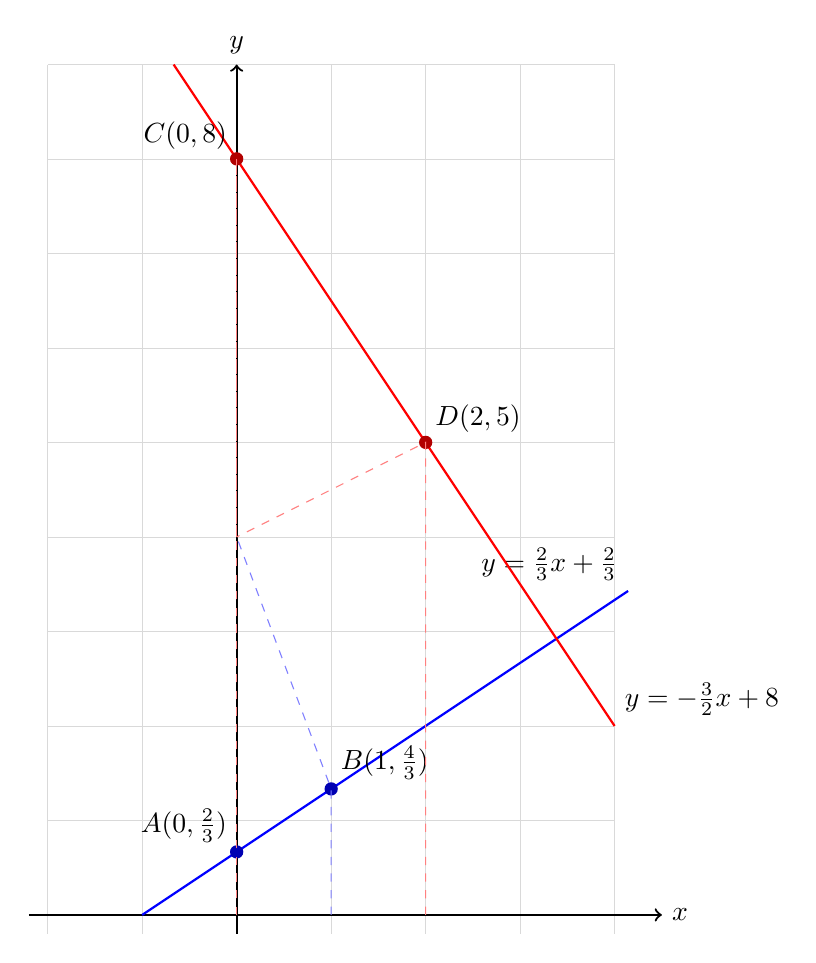
\begin{tikzpicture}[scale=1.2]
    % 1. Cuadrícula de fondo opcional (muy útil para referencia)
    \draw[step=1cm, gray!30, very thin] (-2,-0.2) grid (4,9);

    % 2. Ejes cartesianos
    \draw[->, thick] (-2.2,0) -- (4.5,0) node[right] {$x$};
    \draw[->, thick] (0,-0.2) -- (0,9) node[above] {$y$};

    % 'domain' define el rango de x, y 'samples=2' indica que es una línea recta (dos puntos bastan)
    \draw[thick, blue, domain=-1:5, samples=4.5] plot (\x, {2/3*\x+2/3}) 
        node[above left, black] {$y = \frac{2}{3}x+\frac{2}{3}$};

    \draw[thick, red, domain=-2/3:4, samples=2] plot (\x, {-3/2*\x+8}) 
        node[above right, black] {$y = -\frac{3}{2}x+8$};
    
    \coordinate (P1) at (0,{2/3});
    \fill[blue!70!black] (P1) circle (2pt) node[above left, black] {$A(0,\frac{2}{3})$};
    \draw[dashed, blue!50] (0,0) -- (P1) -- (0,4);
    \coordinate (P2) at (1,{4/3});
    \fill[blue!70!black] (P2) circle (2pt) node[above right, black] {$B(1,\frac{4}{3})$};
    \draw[dashed, blue!50] (1,0) -- (P2) -- (0,4);
    \coordinate (P3) at (0,8);
    \fill[red!70!black] (P3) circle (2pt) node[above left, black] {$C(0,8)$};
    \draw[dashed, red!50] (0,0) -- (P3) -- (0,4);
    \coordinate (P4) at (2,5);
    \fill[red!70!black] (P4) circle (2pt) node[above right, black] {$D(2,5)$};
    \draw[dashed, red!50] (2,0) -- (P4) -- (0,4);

    \end{tikzpicture}
\end{center}
        \item Consideremos $h(x) = f(x-2)$ y $g(x) = h(x) + 2$. Notemos que $h(x)$ es desplazar horizontalmente $f(x)$ dos unidades a la derecha y $g(x)$ es desplazar $h(x)$ dos unidades hacia arriba.
        \begin{equation*}
            g(x) = 
            f(x-2) + 2 = \frac{2}{3} (x-2) +2 
        \end{equation*}
        Por lo que las transformaciones que se le realizan a $f(x)$ es un desplazamiento horizontal dos unidades a la derecha y luego un desplazamiento vertical 2 unidades hacia arriba.
    \end{enumerate}
    \item 
        \begin{enumerate}
            \item Sabemos que el signo del coeficiente $a$ que acompaña a $x^{2}$ determina la orientación de las ramas de la parábola.
            Sea $a$ tal que $f(x) = ax^{2}+bx+c$ si
                \begin{itemize}
                    \item $a>0 \implies $ las ramas de la parábola van hacia arriba.
                    \item $a<0 \implies$ las ramas de la parábola van hacia abajo. 
                \end{itemize}
            Cómo en nuestro caso $a = -\frac{2}{3} < 0$ entonces las ramas de la parábola van hacia abajo.
            \item Sabemos que el vértice tiene coordenadas
            \begin{equation*}
                x_V = -\frac{b}{2a}, \hspace{2cm} y_v = -\frac{b^{2}}{4a}+c
            \end{equation*}
            Tenemos $a=-\frac{2}{3}$ , $b = \frac{4}{3}$ y $c = 2$.
            \begin{equation*}
                x_v = \frac{-\frac{4}{3}}{2(-\frac{2}{3})} = -\frac{4}{3} \cdot -\frac{3}{4} = 1 
            \end{equation*}
            \begin{equation*}
                y_v = \frac{-(\frac{4}{3})^{2}}{4 (-\frac{2}{3})} +2 = -\frac{16}{9}\cdot(-\frac{3}{8}) +2 = \frac{2}{3} + 2 = \frac{2}{8}
            \end{equation*}
            Entonces el vértice es 
            \begin{equation*}
                v = (1, \frac{8}{3})
            \end{equation*}
            La intersección con el eje de las ordenadas es cuando $x = 0$ entonces
            \begin{equation*}
                y = f(0) = -\frac{2}{3}\cdot0^{2}+\frac{4}{3}\cdot0+2 \implies y=2
            \end{equation*}
            \item Apoyándonos en los datos obtenidos y sabiendo que con 3 puntos no alineados se puede graficar una parábola, obtenemos:

            \begin{figure}[H]
            \centering
            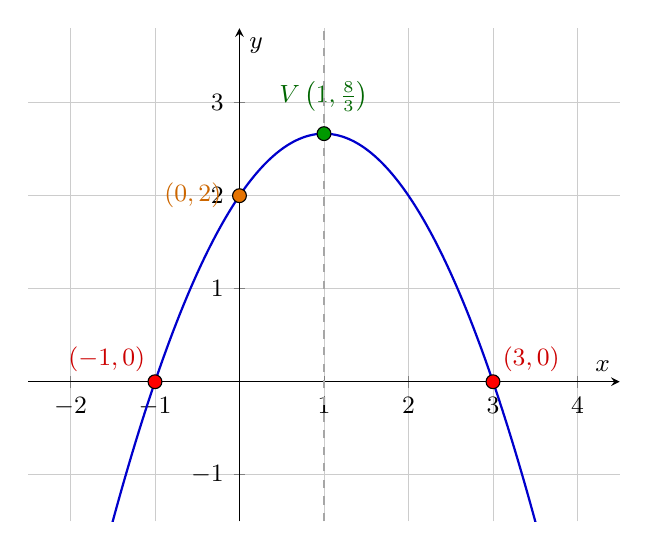
\begin{tikzpicture}
            \begin{axis}[
                width=0.75\textwidth,
                axis lines=middle,
                xlabel={$x$},
                ylabel={$y$},
                xmin=-2.5, xmax=4.5,
                ymin=-1.5, ymax=3.8,
                grid=both,
                grid style={line width=.1pt, draw=gray!20},
                major grid style={line width=.2pt, draw=gray!40},
                tick label style={font=\small},
                label style={font=\small},
                enlargelimits=false
            ]
            
                % 1. Parábola: f(x) = -(2/3)*x^2 + (4/3)*x + 2
                \addplot [domain=-2.2:4.2, samples=100, smooth, thick, blue!80!black] {-(2/3)*x^2 + (4/3)*x + 2};
            
                % 2. Raíces: (-1, 0) y (3, 0)
                \addplot[only marks, mark=*, mark options={fill=red, draw=black, mark size=2.5pt}] 
                coordinates {(-1,0) (3,0)};
                
                \node[anchor=south east, font=\small, color=red!80!black] at (axis cs:-1,0) {$(-1,0)$};
                \node[anchor=south west, font=\small, color=red!80!black] at (axis cs:3,0) {$(3,0)$};
            
                % 3. Intersección eje Y: (0, 2)
                \addplot[only marks, mark=*, mark options={fill=orange!90!black, draw=black, mark size=2.5pt}] 
                coordinates {(0,2)};
                
                \node[anchor=east, font=\small, color=orange!80!black] at (axis cs:-0.1,2) {$(0,2)$};
            
                % 4. Vértice: (1, 8/3)
                \addplot[only marks, mark=*, mark options={fill=green!60!black, draw=black, mark size=2.5pt}] 
                coordinates {(1, 8/3)};
                
                \node[anchor=south, font=\small, color=green!40!black] at (axis cs:1, 2.8) {$V\left(1, \frac{8}{3}\right)$};
            
                % Eje de simetría (opcional)
                \draw[dashed, gray!70] (axis cs:1,-1.5) -- (axis cs:1,3.8);
            
            \end{axis}
            \end{tikzpicture}
            \caption{Gráfica de $f(x) = -\frac{2}{3}x^2 + \frac{4}{3}x + 2$}
            \end{figure}

            \item Para ver analiticamente donde se intersectan una recta y una parabola debemos igualarlas.
            \begin{equation*}
                L=P \implies \frac{2}{3}x +\frac{2}{3} = -\frac{2}{3} x^2+\frac{4}{3}x+2
            \end{equation*}
            Multiplicando todo por $\frac{3}{2}$
            \begin{gather*}
                x + 1 = -x^{2}+2x+3 \\
                x +1 +x^2-2x-3 = 0\\
                x^2-x-2 = 0
            \end{gather*}
            Reconociendo que es una ecuación de segundo grado, podemos buscar sus raíces con Bhaskara, sea $a=1$, $b=-1$ y $c=-2$
            \begin{equation*}
                x_1,x_2 = \frac{-(-1)\pm \sqrt{1-4\cdot1\cdot (-2)}}{2\cdot 1} = \frac{1\pm \sqrt{9}}{2}
            \end{equation*}
            \begin{equation*}
                \implies x_1 =\frac{1+3}{2}=2, \hspace{1cm} x_2 = \frac{1-3}{2} =-1
            \end{equation*}
            Encontramos la coordenada $x$ de los puntos donde intersectan la parábola y la recta. Encontremos la coordenada $y$ de los puntos, evaluando la recta (o la parábola) en $x_1$ y $x_2$

            En $x_1 \implies \frac{2}{3}\cdot 2 + \frac{2}{3} = \frac{6}{3} = 2$.
            
            En $x_2 \implies \frac{2}{3} (-1) + \frac{2}{3} = 0$.

            Por lo tanto los puntos donde la recta $L$ y la parábola se intersectan son $(2,2)$ y $(-1,0)$.
        
        \end{enumerate}
    \item \begin{enumerate}
            \item Sabemos que $P(t) = (x,y) = (cos(t), sen(t))$.
            
            Como $P(t)$ pertenece al tercer cuadrante entonces
            \begin{equation*}
                cos(t) < 0 , \hspace{1cm} sen(t)<0
            \end{equation*}
            Sabemos que $sec(t) = \frac{1}{cos(t)} = -2$ 
            \begin{gather*}
                \implies -2 = \frac{1}{cos(t)} \\
                cos(t) = -\frac{1}{2}
            \end{gather*}
            Sabemos que $cos^2(t)+sen^2(t)= 1 \implies sen^2(t) = 1 - cos^2(t)$.
            \begin{align*}
                sen(t)=& \pm \sqrt{1- (-\frac{1}{2})^{2}}\\ 
                =& \pm \sqrt{1-\frac{1}{4}} \\
                =& \pm \sqrt{\frac{3}{4}}\\ 
                =& \pm \frac{\sqrt{3}}{2}
            \end{align*}
            Como $sen(t) <0 \implies sen(t) = -\frac{\sqrt{3}}{2}$. 
            Entonces $P(t)$ en coordenadas cartesianas queda
            \begin{align*}
                P(t) = (-\frac{1}{2}, -\frac{\sqrt{3}}{2})
            \end{align*}
            Ahora necesito encontrar el ángulo $t$ en radianes. Sabemos que $cos(t) = -\frac{1}{2}$ y $sen(t) = -\frac{\sqrt{3}}{2}$, entonces $t = \frac{4\pi}{3}$ pues dado que $t$ pertenece al tercer cuadrante, el ángulo de referencia es $\frac{\pi}{3}$ y sumando $\pi$ obtenemos $\frac{4\pi}{3}$.
\begin{center}
\begin{tikzpicture}[scale=3.5]
    % 1. Definir el valor del ángulo en grados (puedes cambiarlo, ej: 50)
    \def\angulo{240}

    % 2. Ejes cartesianos
    \draw[->, thin, gray] (-1.3,0) -- (1.3,0) node[right, black] {$x$};
    \draw[->, thin, gray] (0,-1.3) -- (0,1.3) node[above, black] {$y$};

    % 3. Circunferencia unitaria (radio = 1)
    \draw[thick, blue!60!black] (0,0) circle (1cm);

    % 4. Coordenada del punto P usando coordenadas polares (ángulo:radio)
    \coordinate (P) at (\angulo:1);

    % 5. Radio vector desde el origen hasta el punto
    \draw[thick, orange!80!black] (0,0) -- (P);

    % 6. Proyecciones punteadas sobre los ejes (Coseno y Seno)
    \draw[dashed, gray] (P) -- ({cos(\angulo)},0) node[below, black] {$\cos\frac{4\pi}{3}$};
    \draw[dashed, gray] (P) -- (0,{sin(\angulo)}) node[right, black] {$\sin\frac{4\pi}{3}$};

    % 7. Arco que representa el ángulo theta
    \draw[red, thick] (0.3,0) arc[start angle=0, end angle=\angulo, radius=0.3];
    \node at (0.38, 0.18) [red] {$\frac{4\pi}{3}$};

    % 8. Punto P sobre la circunferencia
    \filldraw[red] (P) circle (1pt) node[above right, black] {$P(-\frac{1}{2}, -\frac{\sqrt{3}}{2})$};
\end{tikzpicture}
\end{center}
    
        \item Sabemos que 
            \begin{align*}
            cosec(t) =& \frac{1}{sen(t)} = \frac{1}{-\frac{\sqrt{3}}{2}} = -\frac{2\sqrt{3}}{3} \\
            tg(t) =&\frac{sen(t)}{cos(t)} = \frac{-\frac{\sqrt{3}}{2}}{-\frac{1}{2}} = \sqrt{3}\\
            cotan(t) =&\frac{cos(t)}{sen(t)} = \frac{1}{\sqrt{3}} = \frac{\sqrt{3}}{3} 
            \end{align*}
             \end{enumerate} 
    \item \begin{enumerate}
        \item Podemos identificar dos triángulos rectángulos en la situación problemática:
    \begin{itemize}
        \item Uno de ellos se conforma por el primer punto de observación de Juli ($A$), la punta del edificio a donde mira ($C$) y la base del edificio que se encuentra verticalmente debajo de la punta del edificio ($D$), lo que sabemos de este primer triángulo es que de $A$ a $D$ está contenido el segundo punto de observación de Juli ($B$) que se encuentra a 20 metros de $A$, es decir, $dist(A,D)=dist(A,B)+dist(B,D)=20m + X$ y también conocemos que el ángulo de observación de $A$ a $C$ es de 30 grados.
        \item El segundo triángulo comparte puntos con el anterior excepto $A$, es decir, se conforma por el segundo punto de observación de Juli ($B$), la punta del edificio a donde mira ($C$) y la base del edificio que se encuentra verticalmente debajo de la punta del edificio ($D$), lo que sabemos de este segundo triángulo es lo que definimos en el anterior: $dist(B,D)=X$ y que el ángulo de observación de $B$ a $C$ es de 60 grados.
    \end{itemize}

    \begin{center}
\begin{tikzpicture}[scale=2.5]
    % 1. Definir los vértices del triángulo rectángulo
    \coordinate (A) at (0,0); % Vértice del ángulo recto
    \coordinate (D) at (3,0); % Vértice del ángulo agudo inferior
    \coordinate (C) at (3,2); % Vértice superior

    % 2. Dibujar el contorno del triángulo
    \draw[thick, blue!60!black] (A) -- (D) node[midway, below] {$20 m + X$} 
                                   -- (C) node[midway, above right] {$h$: altura del edificio} 
                                   -- (A) node[midway, left] {$H_1$};

    % 3. Dibujar el símbolo del ángulo recto en el vértice A
    \draw[thick, gray] (2.8,0) -- (2.8,0.2) -- (3,0.2);

    % 4. Dibujar el arco y etiqueta para el ángulo theta en el vértice B
    \draw[red, thick] (0.5,0) arc[start angle=0, end angle=35, radius=0.5];
    \node at (0.75, 0.18) [red] {$30^{\circ}$};

    % 5. Marcar los vértices con letras
    \node at (A) [below left] {$A$};
    \node at (D) [below right] {$D$};
    \node at (C) [above left] {$C$};
\end{tikzpicture}
\end{center}

 \begin{center}
\begin{tikzpicture}[scale=2.5]
    % 1. Definir los vértices del triángulo rectángulo
    \coordinate (B) at (0,0); % Vértice del ángulo recto
    \coordinate (D) at (2,0); % Vértice del ángulo agudo inferior
    \coordinate (C) at (2,2); % Vértice superior

    % 2. Dibujar el contorno del triángulo
    \draw[thick, blue!60!black] (B) -- (D) node[midway, below] {$X$} 
                                   -- (C) node[midway, above right] {$h$: altura del edificio} 
                                   -- (B) node[midway, left] {$H_2$};

    % 3. Dibujar el símbolo del ángulo recto en el vértice A
    \draw[thick, gray] (1.8,0) -- (1.8,0.2) -- (2,0.2);

    % 4. Dibujar el arco y etiqueta para el ángulo theta en el vértice B
    \draw[red, thick] (0.5,0) arc[start angle=0, end angle=45, radius=0.5];
    \node at (0.75, 0.28) [red] {$60^{\circ}$};

    % 5. Marcar los vértices con letras
    \node at (B) [below left] {$B$};
    \node at (D) [below right] {$D$};
    \node at (C) [above left] {$C$};
\end{tikzpicture}
\end{center}

    \item Para calcular la altura del edificio, podemos usar la función tangente que relaciona el ángulo de observación con la altura del edificio y la distancia horizontal desde el punto de observación hasta la base del edificio.
    \begin{itemize}
        \item Para el primer triángulo, tenemos:
        \begin{equation*}
            \tan(30^{\circ}) = \frac{h}{20 + X} \implies h = (20 + X) \cdot \tan(30^{\circ})
        \end{equation*}
        \item Para el segundo triángulo, tenemos:
        \begin{equation*}
            \tan(60^{\circ}) = \frac{h}{X} \implies h = X \cdot \tan(60^{\circ})
        \end{equation*}
   \end{itemize}
   Igualando las dos expresiones para $h$, obtenemos:
    \begin{equation*}
          (20 + X) \cdot \tan(30^{\circ}) = X \cdot \tan(60^{\circ})
     \end{equation*}
     Sustituyendo los valores de $\tan(30^{\circ}) = \frac{\sqrt{3}}{3}$ y $\tan(60^{\circ}) = \sqrt{3}$, tenemos:
     \begin{equation*}
          (20 + X) \cdot \frac{\sqrt{3}}{3} = X \cdot \sqrt{3}
     \end{equation*}
     Multiplicando ambos lados por 3 para eliminar el denominador:
     \begin{equation*}
          (20 + X) \cdot \sqrt{3} = 3X \cdot \sqrt{3}
     \end{equation*}
     Dividiendo ambos lados por $\sqrt{3}$:
     \begin{equation*}
          20 + X = 3X
     \end{equation*}
     Restando $X$ de ambos lados:
     \begin{equation*}
          20 = 2X
     \end{equation*}
     Dividiendo ambos lados por 2:
     \begin{equation*}
          X = 10
     \end{equation*}
     
     Ahora podemos sustituir $X$ en cualquiera de las ecuaciones para encontrar $h$. Usando la ecuación del segundo triángulo:
     \begin{equation*}
          h = X \cdot \tan(60^{\circ}) = 10 \cdot \sqrt{3} 
     \end{equation*}
     
     Por lo tanto, la altura del edificio es $h = 10\sqrt{3}$ metros.


\end{enumerate}
    
        
\end{enumerate}

\end{document}